\documentclass[aspectratio=169,compress]{beamer}
\usetheme[university=bs,faculty=standard]{fibeamer}
\usepackage[utf8]{inputenc}
\usepackage[
  main=english
]{babel}         %% typeset as follows:
%%
%%   \begin{otherlanguage}{italian}   ... \end{otherlanguage}
%%
%% These macros specify information about the presentation
\title{Static Typing for Dynamic Languages:\\
 \large The Case for Set-Theoretic Types and Semantic Subtyping}
\subtitle{\mbox{ }\vspace{6mm}
} %% title page.
\author{Giuseppe CASTAGNA
% \hfill\parbox[t]{.2\textwidth}{
% \footnotesize\it
% Elisir di sì perfetta,\\[-1.5mm]
% di sì rara qualità,\\[-1.5mm]
% ne sapessi la ricetta,\\[-1.5mm]
% conoscessi chi ti fa! 
% }
\\\small
CNRS%(joint work with Guillaume Duboc and José Valim)
}
%% These additional packages are used within the document:
\usepackage[overlay,absolute,
%showboxes
]{textpos}
\usepackage{ragged2e}  % `\justifying` text
\usepackage{booktabs}  % Tables
\usepackage{tabularx}
\usepackage{tikz}      % Diagrams
\usetikzlibrary{calc, shapes, backgrounds}
\usepackage{amsmath, amssymb}
\usepackage{url}       % `\url`s
\usepackage{listings}  % Code listings
\usepackage{setup}
\usepackage{ulem}
\usepackage[cal=boondox,  % heavily sloped
            scr=esstix]   % slightly sloped
           {mathalpha}
\newtagform{purple}{\color{purple}(}{)}
%\frenchspacing

\newcommand{\struct}[1]{\textcolor{lightblue}{#1}}
% Beamer customization%%
\setbeamerfont{frametitle}{shape=\bf,size=\LARGE}
\addtobeamertemplate{frametitle}{\vspace*{-.4cm}}{\vspace*{0.2cm}}

\newenvironment<>{myblock}[1]{%
  \setbeamercolor{block title}{fg=cadmiumgreen,bg=white}%
  \setbeamercolor{block body}{fg=black,bg=white}%
  \setbeamerfont{block title}{size=\large,shape=\bf}
  \begin{block}#2{{#1}\vspace{-1.5mm}}}{\end{block}}

%%%% UNCOMMENT THE FOLLOWING LINE TO REMOVE SLIDE NUMBERS
%\setbeamertemplate{footline}{}

\begin{document}
  \frame[c]{\maketitle}

  %% \AtBeginSection[]{% Print an outline at the beginning of sections
  %%   \begin{frame}<beamer>
  %%     \frametitle{Outline for Section \thesection}
  %%     \tableofcontents[currentsection]
  %%   \end{frame}}

%% ----------------------------------------------------------
%%  SLIDE 2 — Why static typing for dynamic languages?
%% ----------------------------------------------------------
\begin{frame}
\frametitle{Why Static Typing for Dynamic Languages?}

\begin{columns}[T,onlytextwidth]
  \begin{column}{0.48\textwidth}
    \begin{block}{Catch bugs early}\setlength{\baselineskip}{0.85\baselineskip}
      Type errors are found at compile time, before the code ever runs in
      production.
    \end{block}
    \vspace{0mm}
    \begin{block}{Living documentation}\setlength{\baselineskip}{0.85\baselineskip}
      Types describe exactly what a function expects and returns, and they
      are always consistent with the code.
    \end{block}
    \vspace{0mm}
    \begin{block}{Better tooling}\setlength{\baselineskip}{0.85\baselineskip}
      Precise auto-completion, safe refactoring, and IDE navigation all
      rely on type information.
    \end{block}
  \end{column}
  \begin{column}{0.48\textwidth}
    \begin{block}{Safer refactoring}
      Rename or restructure a codebase with confidence: the type
      checker catches every inconsistency.
    \end{block}
    \vspace{3mm}
    \begin{alertblock}{Regulatory compliance}
      EU and US regulations increasingly \textbf{require formally
      certified software} (CRA, NIST guidelines, \ldots).  A
      \emph{\sl sound} type system is a concrete, mechanically verifiable
      step in that direction. No manual-proofs required.
    \end{alertblock}
  \end{column}
\end{columns}

\end{frame}

%% ============================================================
%%  EXTRA SLIDE — Socio-economic and technical context
%%  Insert into main.tex at the desired position
%% ============================================================

\begin{frame}
\frametitle{Socio-Economic and Technical Context}
\vspace{-3mm}
\begin{columns}[T,onlytextwidth]
  %% ---- left column ----------------------------------------
  \begin{column}{0.45\textwidth}
    \begin{block}{Technical challenges}\setlength{\baselineskip}{0.9\baselineskip}\setlength{\leftmargini}{1.2em}
      \begin{itemize}\setlength{\itemsep}{8pt}
        \item Dynamic languages (JavaScript, PHP, Elixir, Python) are
              widely \textbf{used for critical and distributed infrastructures},
              precisely because of their flexibility
        \item They are prone to \textbf{hidden vulnerabilities} and are
              \textbf{hard to maintain at scale}
        \item \textbf{Major safety risks} for systems that require formal
              correctness guarantees
      \end{itemize}
    \end{block}
  \end{column}

  %% ---- right column ---------------------------------------
  \begin{column}{0.51\textwidth}
    \begin{block}{Socio-economic challenges}\setlength{\baselineskip}{0.9\baselineskip}
      \setlength{\leftmargini}{1.2em}
      \begin{itemize}\setlength{\itemsep}{11pt}
        \item Large corporations (Microsoft, Meta, \ldots) have created
              \textbf{proprietary} typed solutions for JavaScript and
              PHP, but these remain language-specific and lack formal
              guarantees
        \item Full rewrites into statically typed languages require
              \emph{years of work} and major resources
        \item A solution is needed that offers formal guarantees, is \textbf{gradual} and \textbf{automated},
              and remains \textbf{open and accessible}
      \end{itemize}
    \end{block}
  \end{column}

\end{columns}

\end{frame}

%% ----------------------------------------------------------
%%  SLIDE 3 — The challenge
%% ----------------------------------------------------------
\begin{frame}
\frametitle{The Challenge: Dynamic Code Does Not Fit Classic Types}

Dynamic languages are expressive \emph{because} they use programming
patterns that traditional type systems cannot describe:

\bigskip

\begin{block}{1. \; Non-uniform data structures / branching}\setlength{\baselineskip}{0.8\baselineskip}
  A dedicated tag field in a record or a tuple is used as a discriminant to determine the type of the remaining values (tagged unions).   \textbf{Union types and singleton types} are needed.
\end{block}

%\bigskip

\begin{block}{2. \; Overloading (ad hoc polymorphism)}\setlength{\baselineskip}{0.8\baselineskip}
  The same function behaves differently depending on whether it receives, say,
  an integer or a string.
  \textbf{Intersection types} are needed.
\end{block}

%\bigskip

\begin{block}{3. \; Pattern matching}\setlength{\baselineskip}{0.8\baselineskip}
  Branches match specific shapes of data; only certain values can reach
  each branch.
  \textbf{Negation types} are needed to track what has already been
  eliminated.
\end{block}

\end{frame}


% \begin{frame}
% \transdissolve<2->
% \frametitle{Set-theoretic types}

% We consider the following possibly recursive types:

% {\Bl$$\T\ ::=\  \Bool\,\mid\,\Int\,\mid\,\pair\T\T\,\mid\,\T\To\T \,\mid\,{\color{darkgreen}\T\Or\T}\,\mid\,{\color{darkgreen}\T\!\And\!\T} \,\mid\, {\color{darkgreen} \neg\T}\,\mid\,{\color{darkred}\Any}\,\mid\,{\color{darkred}\Empty}\,\color<1>{white}\mid\,~\textcolor<2>{magenta}{\alpha} \color<2>{white}\,\mid\, \color<3>{magenta}{c} $$}

% \pause\pause\pause\pause\pause
% \bigskip

% \textbf{Necessary to precisely capture the programming style used with dynamic languages:}
% \begin{enumerate}
% \item non-uniform structures/branching (union types, singletons)
% \item overloading (intersection types)
% \item pattern matching (negation types, ...)
% \end{enumerate}


% \textbf{\color<-6>{white}\color<7>{darkslateblue}Let us see each point more in detail}

% \bigskip

% \vfill

% \small\color{gray} Note: henceforward I will sometimes use $\Bl\T_1\texttt{|}\T_2$ to denote $\Bl\T_1\Or\T_2$

% \only<2>{\begin{textblock}{5}(0,0)
% 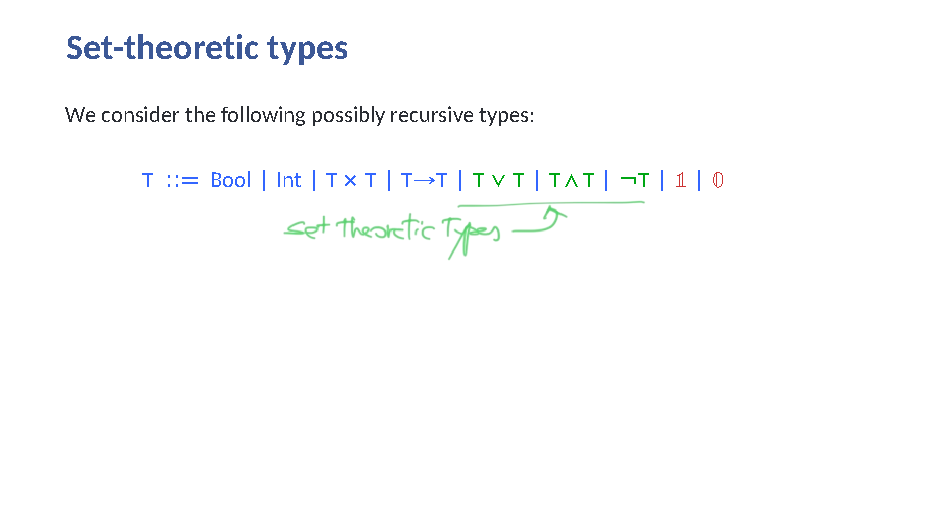
\includegraphics[scale=1]{images/slide-settheore.pdf}
% \end{textblock}}
% \only<3>{\begin{textblock}{5}(0,0)
% 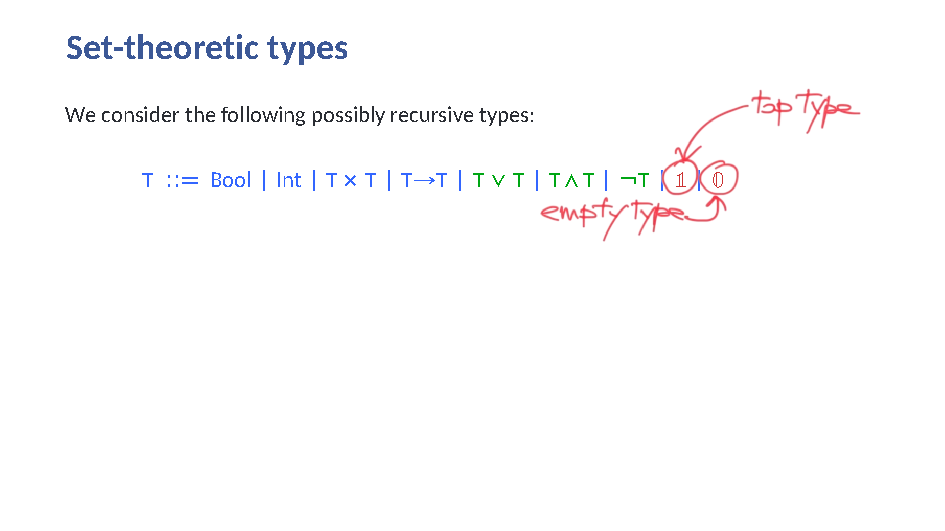
\includegraphics[scale=1]{images/slide-topbottom.pdf}
% \end{textblock}}
% \only<4>{\begin{textblock}{5}(0,0)
% 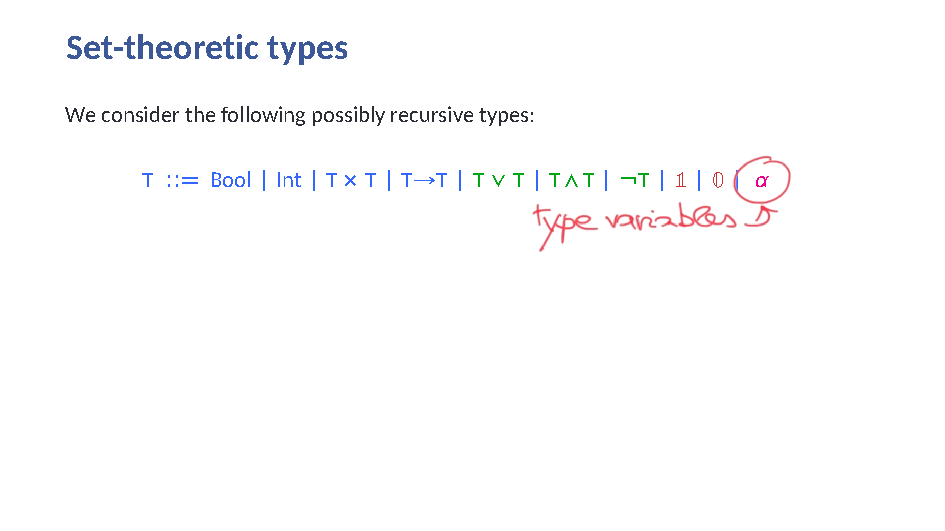
\includegraphics[scale=1]{images/slide-variables.pdf}
% \end{textblock}}
% \only<5>{\begin{textblock}{5}(0,0)
% 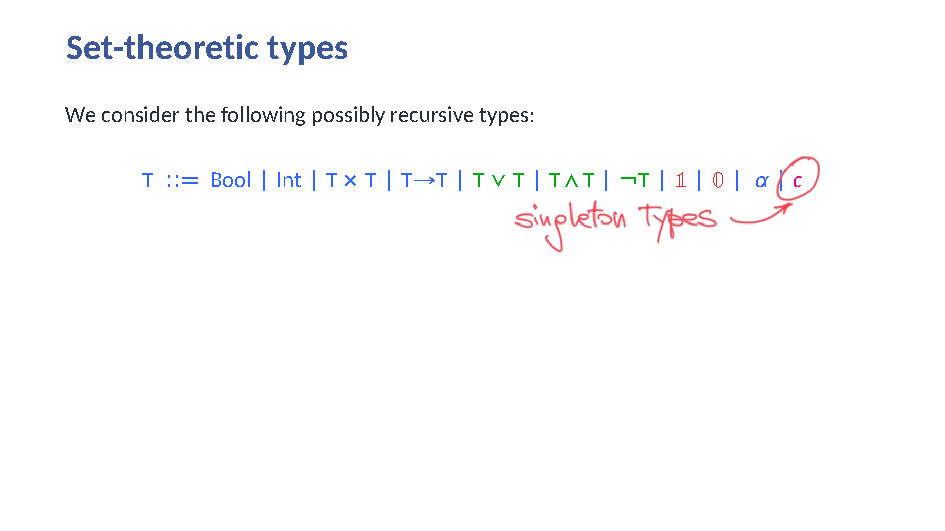
\includegraphics[scale=1]{images/slide-singleton.pdf}
% \end{textblock}}
% \end{frame}

\subsection{Branching, overloading, and pattern matching}

\begin{frame}[fragile]\transdissolve
\frametitle{1. Branching and discriminated unions}\vspace{-7mm}
\small
\begin{minted}{typescript}
type Status = "pending" | "success" | "error";
type Result = string | number | boolean;
function processStatus(input: Status): Result {
  switch (input) {
    case "pending":
      return "Processing...";       // returns string
    case "success":
      return 200;                   // returns number
    case "error":
      return false;                 // returns boolean
    default:
      return "Unknown status";      // returns string
  }
}
\end{minted}
\pause
\vspace{-10mm}

% Discriminated unions are a common pattern in dynamic languages to handle different types of data structures that share some common properties.
\begin{minted}{typescript}
type PaymentMethod = 
  | { medium: "credit_card"; cardNumber: string; cvv: string }
  | { medium: "paypal"; email: string }
  | { medium: "transfer"; accountNumber: string; routingNumber: string };
\end{minted}
\end{frame}



\begin{frame}[fragile]\transdissolve
  \frametitle{2. Overloading: basic use}
 \structure{\bf Aka \emph{ad hoc} polymorphism: functions that execute different code on arguments of different types}


\begin{minted}{typescript}
function double (x) {
    return (typeof(x) === "number") ? 2*x : x.concat(x);
}
\end{minted}
\textcolor<4>{red}{If applied to an integer returns an integer, if applied to a string returns a string}
  \pause
\begin{exampleblock}{Use set-theoretic types}
  \begin{itemize}
    \pause
     \item Naive solution: union types
       \centerline{\pb{(number|string)$\to$(number|string)}}
       \pause\pause
     \item Better solution: intersection types
       \centerline{\pb{\color<6>{darkred}(number$\to$number) \& (string$\to$string)}}
  \end{itemize}
\end{exampleblock}
\end{frame}


\begin{frame}[fragile]
\frametitle{2. Overloading: advanced use}\vspace{-7mm}
\begin{minted}{typescript}
function toBoolean(x) {
    if (x === 0 || x === "" || x == null || Number.isNaN(x)) return false;
    return true;
}

function logicalOr(x, y) {
    if (toBoolean(x)) return x; return y;
}
\end{minted}
\pause
\vspace{-5mm}


\begin{exampleblock}{Fine grained typing to capture the code semantics}\setlength{\baselineskip}{0.9\baselineskip}
\color{typeBlue}
\tt
type Falsy = 0 | "" | null | undefined | NaN;

type Truthy = $\neg$Falsy;

toBoolean : (Truthy $\to$ true)  $\wedge$ (Falsy $\to$ false)

logicalOR : $\forall \alpha,\beta.\, ((\alpha{\wedge}$Truthy$\,\times\,\texttt{Any}$)$ \to \alpha$)  $\wedge$ ((Falsy$\times \beta$)$\,\to \beta$)

\end{exampleblock}
\end{frame}




\begin{frame}[fragile]
\frametitle{3. Precise typing of pattern matching (I)}
Consider the following possibly recursive types:
{\Bl$$\T\ ::=\  ~\textcolor{magenta}{\alpha} \,\mid\, \textcolor{magenta}{c} \,\mid\,\Bool\,\mid\,\Int\,\mid\,\pair\T\T\,\mid\,\T\To\T \,\mid\,{\color{darkgreen}\T\Or\T}\,\mid\,{\color{darkgreen}\T\!\And\!\T} \,\mid\, {\color{darkgreen} \neg\T}$$}
\pause
And let us type the following pattern matching expression:
 
\hspace*{5mm}{\Bl$\texttt{ match }  e  \texttt{ with } p_1 \texttt{ -> } e_1 \texttt{ | } p_2\texttt{ -> } e_2$}

where patterns are defined as follows:
\centerline{$\Bl p ::= x \ \mid\  \patpair{p}{p} \ \mid\ \pator{p}{p}\ \mid\ {p}\,\textsf{and}\,{p} $}
\pause
If we interpret types as set of values
\centerline{$\Bl
t = \{ v\mid v\text{ is a value of type }t\}$}
\pause
then \textbf{\color{darkslateblue}the set of all values that match a pattern is a type}
\centerline{\color{magenta}
$\accept{p} = \{ v\mid v\text{ is a value that matches }p\}
$}

\textbf{\color{darkslateblue}(the accepted type of pattern $p$)}.
\end{frame}



\begin{frame}
\frametitle{3. Precise typing of pattern matching (II)}\transdissolve<10>

\textbf{Boolean type connectives are needed to type pattern matching:}

\pause
\smallskip

    \hspace*{5mm}{\Bl$\texttt{ match }  e  \texttt{ with } p_1 \texttt{ -> } e_1 \texttt{ | } p_2\texttt{ -> } e_2$}\pause

   \smallskip

Suppose that $\Bl e:\T$\\[-2mm]

\pause

  - To infer the type $\Bl\T_1$ of $\Bl e_1$ we need {\color{blue}$\T{\color<8->{magenta}\mypmb<8->{\And}}\accept{p_1}$};

\pause

  - To infer the type $\Bl\T_2$ of $\Bl e_2$ we need {\color{blue}$(\T{\color<8->{magenta}\,\mypmb<8->{\backslash}}\accept{p_1}){\color<8->{magenta}\mypmb<8->{\And}}\accept{p_2}$;}\hspace*{18mm} {\textcolor{gray}{\small($\T_1\setminus\T_2$ stands for $\T_1\!{\And}\!\textcolor<8->{magenta}{\neg}{\T_2}$)}}

\pause

  - The type of the match expression is {\color{blue}$\T_1{\color<8->{magenta}\mypmb<8->{\Or}} T_2$ }.

\pause

  - Pattern matching is exhaustive if $\color{blue}\T\leq\accept{p_1}{\color<8->{magenta}\mypmb<8->{\Or}}\accept{p_2}$;


\pause\pause
\textbf{Formally:}
\vspace{-2mm}
\begin{mathpar}\Bl
\infer[{[Match]}]
{\Gamma\vdash e:\T\and\Gamma, \T\!\!\And\!\!\accept{p_1\!}/p_1\vdash e_1:\T_1\and \Gamma, \T\setminus\accept{p_1\!}/p_2\vdash e_2:\T_2}
{\Gamma\vdash \texttt{match } e \texttt{ with }p_1 \texttt{->} e_1 \texttt{ | }p_1 \texttt{->} e_2 : \T_1\Or\T_2 }\mbox{\small($\T\leq\accept{p_1\!}\Or\accept{\!p_2\!}$)}
\end{mathpar}
\vspace{-4mm}

\small\color{gray}
where $\Bl \T/p$ is the type for the capture variables in $\Bl p$ when it is matched against values in $\Bl \T$.

\only<10>{\begin{textblock}{5}(0,0)
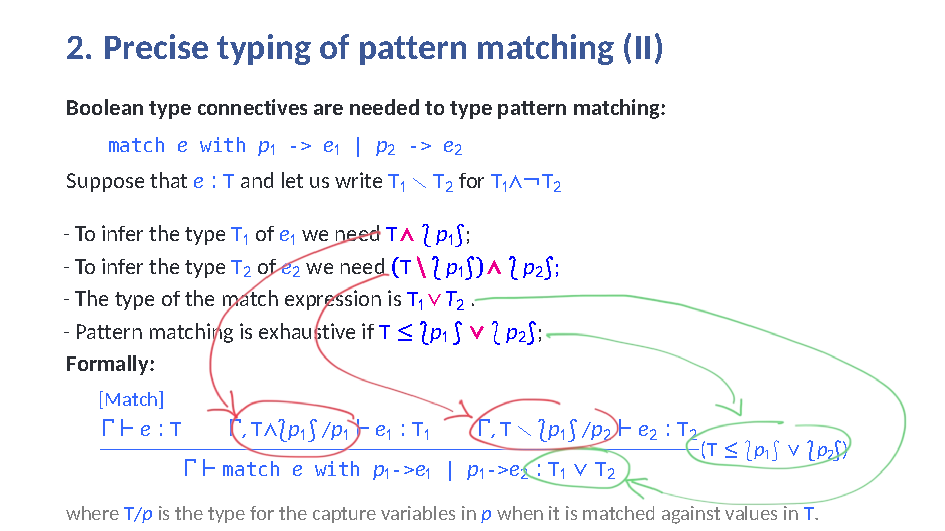
\includegraphics[scale=1]{images/slide-caseexp.pdf}
\end{textblock}}
\end{frame}

\subsection{Semantic subtyping}
\begin{frame}
\frametitle{Semantic subtyping} \vspace{-5mm}

Many dynamic languages support union and intersection types: TypeScript, Flow, Hack, Python, Julia, and Ceylon. Negation types are less common: TypeScript (with the `Exclude` utility type) and Scala (with `Not` type constraints).

\pause\smallskip

\textbf{What differentiates our approach is the use of \emph{semantic subtyping}: i.e., the use of type semantics to define  the subtyping relation for union, intersection, and negation types.}

\smallskip \pause
\begin{block}{Why not just write down subtyping rules?} \setlength{\baselineskip}{0.8\baselineskip}
  Many languages do exactly that — and end up with an incomplete,
  fragile system: e.g., 
  $\neg(A\vee B)$ not a subtype of $\neg A\wedge\neg B$.  With semantic subtyping it comes for \textbf{free}
\end{block}\pause
\textbf{\textcolor{darkslateblue}{How does it work?}}
\begin{enumerate}
  \item<4-> Define a set-theoretic interpretation of types as sets of values
  \item<5-> Define union, intersection, and negation types as set-theoretic operations
  \item<6-> Define the subtyping relation as a set-theoretic inclusion relation
  \item<7-> Deduce from this how to decide the subtyping relation and compute type operators
  \end{enumerate}

\end{frame}


%% ----------------------------------------------------------
%%  SLIDE 7 — Gradual typing
%% ----------------------------------------------------------
\begin{frame}
\frametitle{Gradual Typing: No Big-Bang Migration}\vspace*{-3mm}

\textbf{\color{darkslateblue}Two non-negotiable requirements for real-world adoption by existing languages:}\\
\textbf{\hspace*{.4mm}1.} You do not have to type your entire codebase at once.\\
\textbf{2.} Types do not modify the run-time semantics of existing programs.


\pause 

\medskip

\begin{block}{The \texttt{dynamic()} type}\setlength{\baselineskip}{0.85\baselineskip}
  A special type that represents a value whose type is only checked at
  run time.  It acts as an escape hatch that lets untyped and typed code
  coexist seamlessly.
\end{block}

\smallskip

\begin{enumerate}
  \item Start with an \emph{untyped} codebase — no annotations required.
  \item Add type annotations incrementally, module by module or
        function by function.
  \item Typed and untyped code interoperate without restriction.
  \item As coverage grows, more errors are caught statically.
  \item The end goal — a fully typed codebase — gives the same safety
        guarantees as a fully static system, \emph{at your own pace}.
\end{enumerate}

\end{frame}

\begin{frame}
\frametitle{Putting the theory to work: Elixir}
\begin{itemize}[<+->]
\item Elixir is a dynamic language with a strong emphasis on metaprogramming
\item It is a functional language with a syntax similar to Ruby
\item It is built on top of the Erlang VM, which provides a powerful runtime system for distributed and fault-tolerant applications
\item It has a rich ecosystem of libraries and frameworks and a strong community of nearly 100K developers (with the highest median salaries cf.\  2024 Stack Overflow survey)
\item It is used in production by companies like Discord, Pinterest, PepsiCo, ...
\item Since 2021 we have been collaborating with José Valim, the creator of Elixir, and the Dashbit team to develop a type system for Elixir. (CIFRE industrial PhD thesis)
\item The static type system is based on the set-theoretic types we have developed in the past years and being gradually integrated into the Elixir compiler since version 1.17 in 2024 (the current version is 1.19).
\end{itemize}
\end{frame}

\begin{frame}[fragile]
\frametitle{Status of the Integration}\vspace{-3mm}
\begin{itemize}
\item Very positive feedback from developers on versions 1.17, 1.18, and 1.19
\item No syntactic changes required to Elixir code was particularly appreciated
\item Uncovered previously hidden errors without significant overhead
\item Found issues in all major projects: Phoenix, Livebook, Postgrex, and Flame.\\[-1mm]  They persisted undetected in production, sometimes for years
\end{itemize}

\bigskip\pause

\begin{block}{Real-world Bug Discoveries}
\begin{itemize}
    \setlength{\itemsep}{0pt}
\item \textbf{Phoenix}: Critical type mismatch in \code{String.to_atom/1} \hfill\small (deployed on 14,600+ websites)
\item \textbf{Postgrex}: 15 lines of dead code removed
\item \textbf{Flame}: 2 dead code paths found via guard analysis
\item \textbf{Live-view}: 6 lines of dead code removed
\item \textbf{Remote}: detected a critical type mismatch application in Remote codebase (25K modules)\\ undetected by tests because in an error branch that is rarely executed.\vspace{-1mm}
\end{itemize}
\end{block}
\end{frame}

\begin{frame}[fragile]
\frametitle{\mbox{Several Languages use (more or less) Semantic Subtyping:}}
\hspace*{-0.8em}%
\begin{minipage}{1.06\textwidth}
  \setlength{\leftmargini}{1.9em}
\begin{itemize}\setlength{\itemsep}{2pt}  \setlength{\rightmargin}{-12pt} % reduce right margin (use full width)

  \item \textbf{Elixir} — full type system in the compiler since v1.17
        (2024), actively used in production
        % (Discord, Pinterest,PepsiCo, \ldots)

  \item \textbf{Python (\textsf{ty})} — Astral's high-performance type
        checker reuses data-structures and optimisations developed for
        Elixir, and is migrating to a full semantic subtyping implementation.

  \item \textbf{Ballerina} (WSO2) — uses semantic subtyping since its
        Swan Lake release

  \item \textbf{Luau} (Roblox) — falls back to semantic subtyping when
        syntactic subtyping is insufficient

  \item \textbf{Erlang} — \emph{RPTU} (Kaiserlautern) develops \textsl{Ethylizer} which reconstructs set-theoretic types  for unannotated
        code by using our semantic subtyping algorithms and techniques; \\
        \emph{Meta} develops \textsl{eqWAlizer} to type WhatsApp's Erlang codebase, building on our semantic-subtyping-based gradual typing.

  \item \textbf{R} — \emph{U.\ Karlova} (Prague) is developing a type system for R
        based on semantic subtyping

  \item \textbf{Julia} — core developers cite semantic subtyping as
        direct inspiration for Julia's type system

  \item \textbf{CDuce} and its spin-offs SSTT and MLsem — the original
        theoretical proving grounds
\end{itemize}
\end{minipage}
\end{frame}


\begin{frame}[fragile]
\frametitle{Future work}\vspace{-2mm}

\textbf{\color{darkslateblue}Types for the Elixir Module System:}\\
Currently, only the type \code{module()} is supported, while we want a finer-grained typing of functions manipulating modules. We are developing solutions applicable to other languages.
% \vspace{-5mm}
% \begin{block}{\vspace{-25mm}}
% \begin{minted}{elixir}
% !\spec! (X: Stack[el=bool], sx: X.stack, Y: Stack[el=bool], sy: Y.stack) -> Y.stack
% def move(X, sx, Y, sy), do: Y.push(sy, X.top(sx))   
%\end{minted}
%\end{block}

\bigskip
\textbf{\color{darkslateblue}Record types comprehensions:}\\
We want to type standard library functions that manipulate records with \emph{first-class} keys, such as \code{Map.intersect/2} and \code{Map.reject/2}.
% \definecolor{typeconstructorgreen}{rgb}{0.0, 0.5, 0.25}  % Nice green for type constructors
% \definecolor{keyvarblue}{rgb}{0.1, 0.3, 0.7}              % Nice blue for key variables
% \newcommand{\keyof}[1]{\textcolor{typeconstructorgreen}{\mathsf{keyof}}(#1)}
% \newcommand{\tvar}{\textcolor{keyvarblue}{\boldsymbol{\theta}}}
% \begin{tabular}{@{}l@{\;\;}l@{\;\;}l@{}}
%  \texttt{intersect/2}
%   & $(\alpha,\, \beta) \to \%\{\,\tvar \in \keyof{\alpha} \land \keyof{\beta} \mid \beta[\tvar]\,\}\quad\texttt{when } \alpha,\beta\texttt{:map()}$  \\[6pt]
% \texttt{reject/2}
%   & $(\alpha, ((\keyof{\alpha} \to \texttt{term}) \,\wedge\, ( \keyof{\alpha}\wedge\beta)\to\neg\texttt{truthy})) \to $\\
%   &\qquad\qquad\qquad\qquad
%      $\%\{\, \tvar\in \keyof{\alpha}\setminus\beta \mid \alpha[\tvar]\,\} \quad\texttt{when } \alpha\texttt{:map()}$\\[3pt]
% \end{tabular}

\bigskip
\textbf{\color{darkslateblue}Types for processes and message passing:}
Currently, only the type \code{pid()} is supported.

In collaboration with \emph{Università degli Studi di Bologna} (Italy) and \emph{Université d'Evry} (France), we are working on typing processes with the set of messages they can receive and, later, we plan to introduce Mailbox types, to ensure liveness properties.

\end{frame}
\begin{frame}
\frametitle{Future work}\vspace*{-5mm}

\textbf{\color{darkslateblue}Tooling:} We are developing migration tools, IDEs, error messages, .... In particular, in collaboration with \emph{Ca' Foscari} (Venice), we are  feeding LLMs with automatic translations of TypeSpecs into Elixir Types together with the type errors they produce to improve the quality of LLM-generated type annotations and error messages.

\bigskip\medskip

\textbf{\color{darkred}Application to Ruby:} We are collaborating with \textbf{NII} and members of the Ruby team to apply our gradual typing solutions to Ruby, which has a syntax similar to Elixir but is object-oriented and has a more complex type system (with classes, modules, \ldots).


\end{frame}



%% ----------------------------------------------------------
%%  SLIDE 10 — Why this is the most promising approach
%% ----------------------------------------------------------
\begin{frame}
\frametitle{A Proven Approach}

\begin{enumerate}\setlength{\itemsep}{4pt}

  \item \textbf{\color{darkslateblue}Faithful to the semantics.}
    $T_1 \leq T_2$ means exactly $\llbracket T_1\rrbracket \subseteq
    \llbracket T_2\rrbracket$ — no axioms, no approximations.

  \item \textbf{\color{darkslateblue}Designed for dynamic idioms.}
    Overloading, pattern matching, and non-uniform branching are all
    described \emph{naturally}, without awkward workarounds.

  \item \textbf{\color{darkslateblue}Gradual typing.}
    Works incrementally.  No flag day, no forced full rewrite.  Start
    with nothing and add types where they help.

  \item \textbf{\color{darkslateblue}Proven in production.}
    Already integrated in Elixir, Python, Ballerina, Erlang.  Finding
    real bugs in real codebases \emph{today}.

  \item \textbf{\color{darkslateblue}Solid theoretical foundations.}
    Backed by 15+ years of peer-reviewed work (JACM, POPL, ICFP,
    OOPSLA).  

  \item \textbf{\color{darkslateblue}Supports formal certification.}
    Soundness is proved, not just tested — directly relevant to
    regulatory requirements for certified software.

\end{enumerate}

\end{frame}


%% ----------------------------------------------------------
%%  SLIDE 11 — Takeaways
%% ----------------------------------------------------------
\begin{frame}
\frametitle{Takeaways} \vspace*{-6mm}

\begin{enumerate}[<+->]\setlength{\itemsep}{6pt}

  \item Dynamic languages need static typing — for correctness, tooling,
        and regulatory confidence.

  \item Traditional type systems were not built for dynamic idioms.
        A new model is needed.

  \item Set-theoretic types with semantic subtyping provide that model:
        \emph{expressive, correct, and well-founded}.

  \item Gradual adoption means no disruption — start typing today,
        incrementally.

  \item Already validated across 8+ languages and real-world production
        codebases.

  \item \textbf{\color{darkslateblue}The theory is solid —and still advancing. The practice is proven. The adoption is growing}

\end{enumerate}

\end{frame}

\end{document}
